\section{Results}
\label{sec:results}
In order to understand how a given classifier with its specific properties (e.g. those that take a `winner takes all' approach compared to those that provide balanced classifications across types) performs in different metric schemes, we simulate the responses of both the log-loss metric and the Brier score as a function of isolated `systematic effects' imposed on various classifier baselines.
What we mean by systematic is some alteration to the standard classifier that could affect its performance.  We outline these systematics below.

\subsection{Mock classifier systematics}
\label{sec:mockresults}

In Figure~\ref{fig:cruise}, we illustrate shows the effect of adding each of four forms of error to a classification scheme that performed perfectly at classifying objects of a given type (prior to the systematic being added).
The four systematics include changing the classification from perfect to almost perfect as described in Section~\ref{sec:accuratedata}, subsuming the classifications of class $m'$ for another class $\tilde{m}$ (labelled by `subsumed'), changing the classification from perfect to wholly uncertain, and making the classification more `noisy', which is by a reduction in the contribution of the classifier by a factor of $s=2,$ as described in Section~\ref{sec:accuratedata}.
In each case, the metric weights are assumed to be flat.
The log-loss and Brier scores behave very consistently, with the log-loss more affected than the Brier score for systematics in which the class $m'$ is subsumed by a different class (top right panel), however the effect is reasonably small.
This shows that for a given metric (log-loss/Brier) and classification scheme, the metrics are stable to the introduction of systematic changes in the classifications.
Both metrics are appropriate for singling out a classifier that enables any class to subsume other classes, thereby confirming that the cruise control classifier will not in general outscore a classifier that avoids subsuming.

\begin{figure}
	\begin{center}
		\label{fig:cruise}
		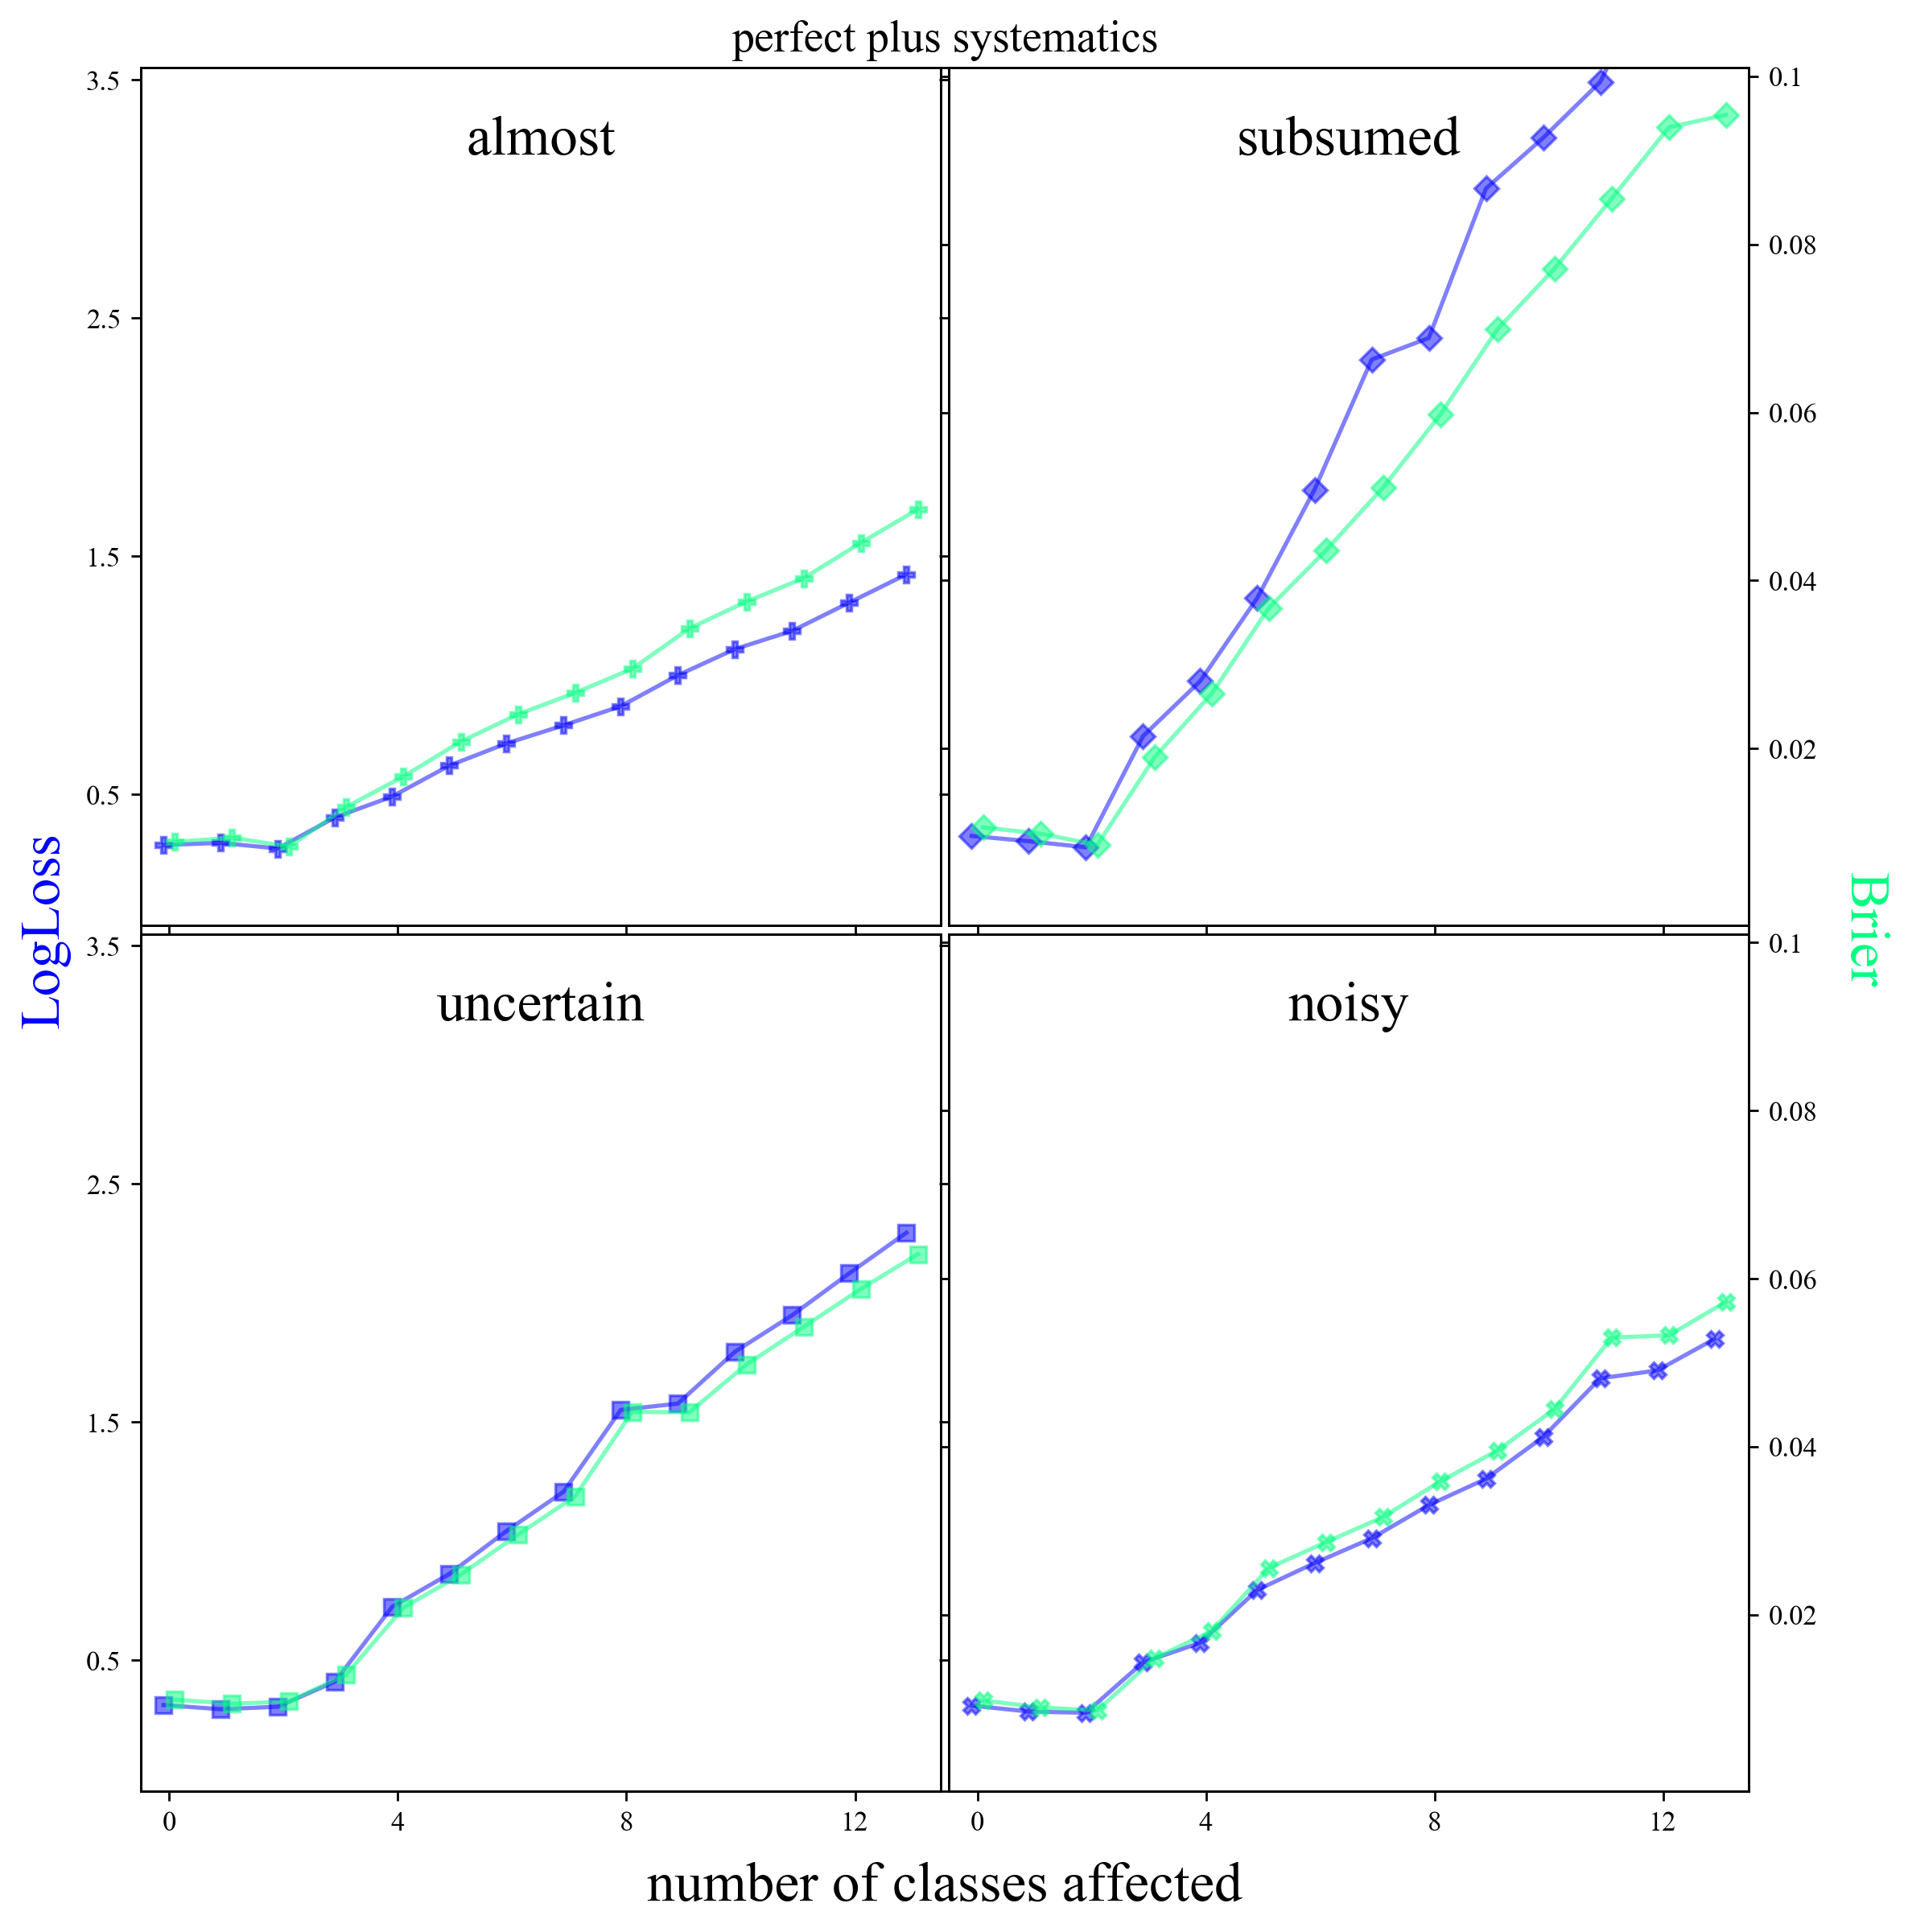
\includegraphics[width=0.5\textwidth]{./fig/systematics_onlyperfect.png}
		\caption{Systematic effects added to the perfect classifier.
		The log-loss and Brier scores (left and right $y$ axes, respectively) are shown for classifiers that are ``perfect' aside from the indicated systematic (panels) as a function how many classes are affected by the systematic (on the $x$-axis), beginning with the lowest population classes.
		The two metrics behave very similarly to one another and have high sensitivity to a subsuming classifier.}
	\end{center}
\end{figure}

It is common for `tunnel classifiers' or those that follow a `winner takes all' approach to dominate classification schemes, and large, unbalanced data sets can be especially prone to this.
As such, one approach is to require a threshold of classification of all classes in order to assign a winner in any classification challenge.
We introduced weighting of per-class metrics to discourage `tunnel vision' and `cruise control' classifiers that can ignore classes other than the most common and nonetheless perform well by a metric.
Figure~\ref{fig:popweight}, shows the impact of weighting the metric by number of objects in the class.
The points show different classification schemes, and all points are coloured by the change in the weighting, dependent on the size of the population class being classified.
The tunner classifier has a consistently low Brier score and log-loss score (bottom left corner of the plot), only increasing its Brier score once the weighting is severe.
Conversely, the cruise control classifier prefers to be heavily weighted by the number of objects in the class, but under-performs relative to the tunnel for all values of the weights.

\begin{figure}
	\begin{center}
		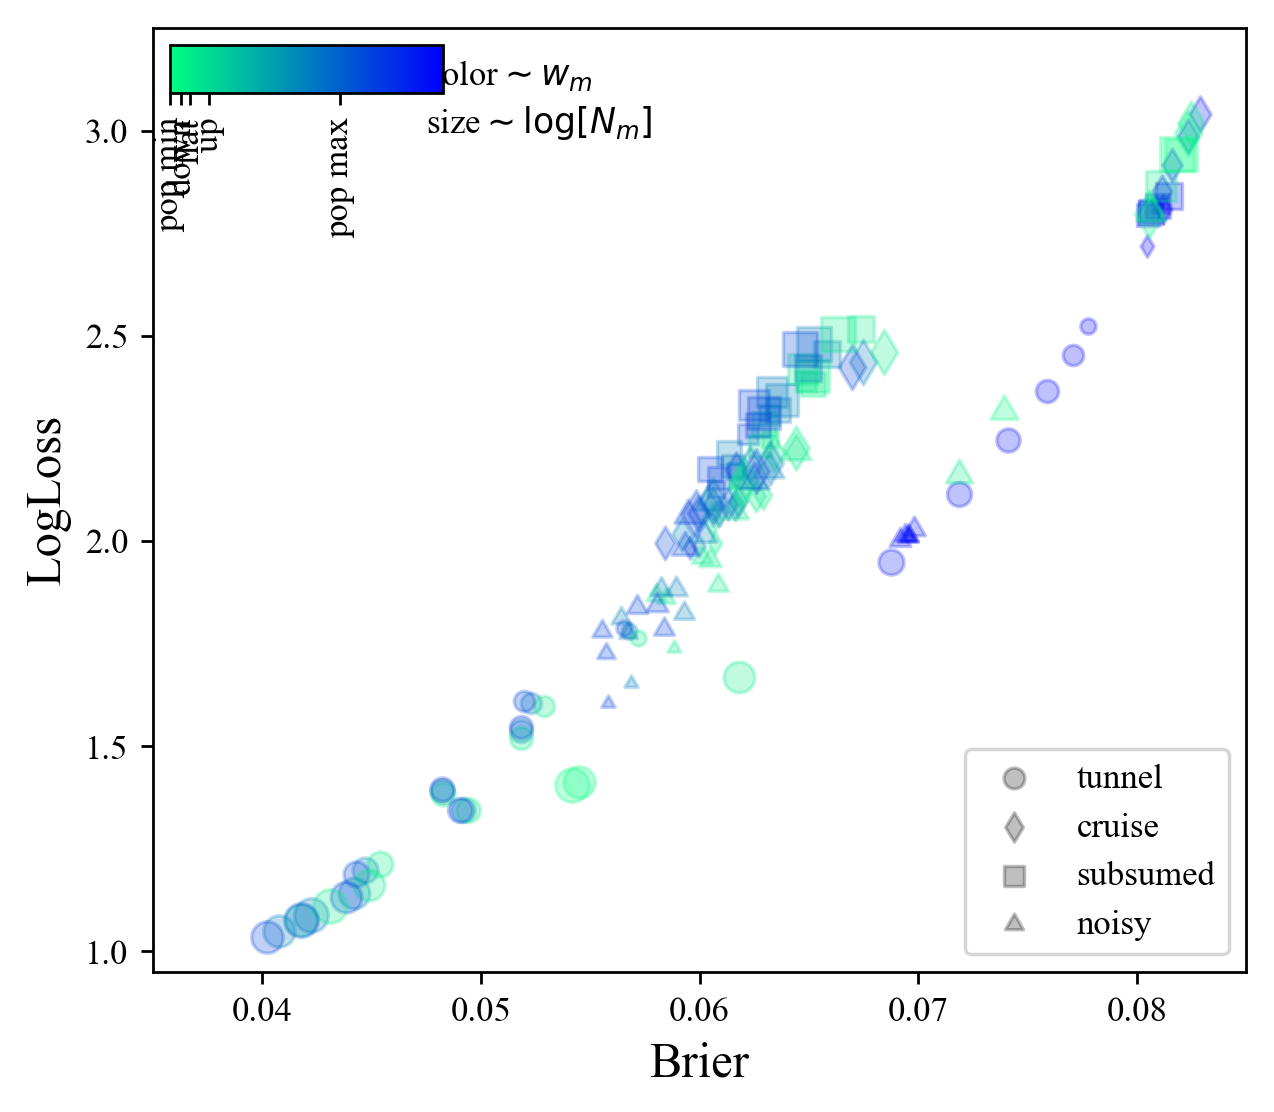
\includegraphics[width=0.5\textwidth]{./fig/all_effects_isolated.png}
		\caption{Classification algorithm performance on the log-loss and Brier scores. We evaulate a few characteristic classification approaches (indicated by the symbols) in the log-loss-Brier metric space (where a low score indicates a more favourable classification).
		The points are coloured by weights which depend on the overall number of objects in the class \textbf{[are the weights getting more extreme, but we are keeping the N in each bin constant? Make this clearer.]}.
		In almost all cases, the tunnel classifier out performs the other classification schemes.
		When considering a method of converting from a Brier score to a finall `winner' of the classification challenge, care must be taken to ensure that all approaches do reasonably well at classifying more than one object.
		This thresholding procedure is discussed in the text \label{fig:popweight}}
	\end{center}
\end{figure}

\textbf{Ashish to reaplce/add more here?}
%\aim{Preliminary results indicate weighting will be very important for preventing the tunnel vision classifier from winning. It may be necessary to a priori anticipate which classes will have to be most strongly protected from this systematic via upweighting them.}

%\begin{figure}
%	\begin{center}
%		% 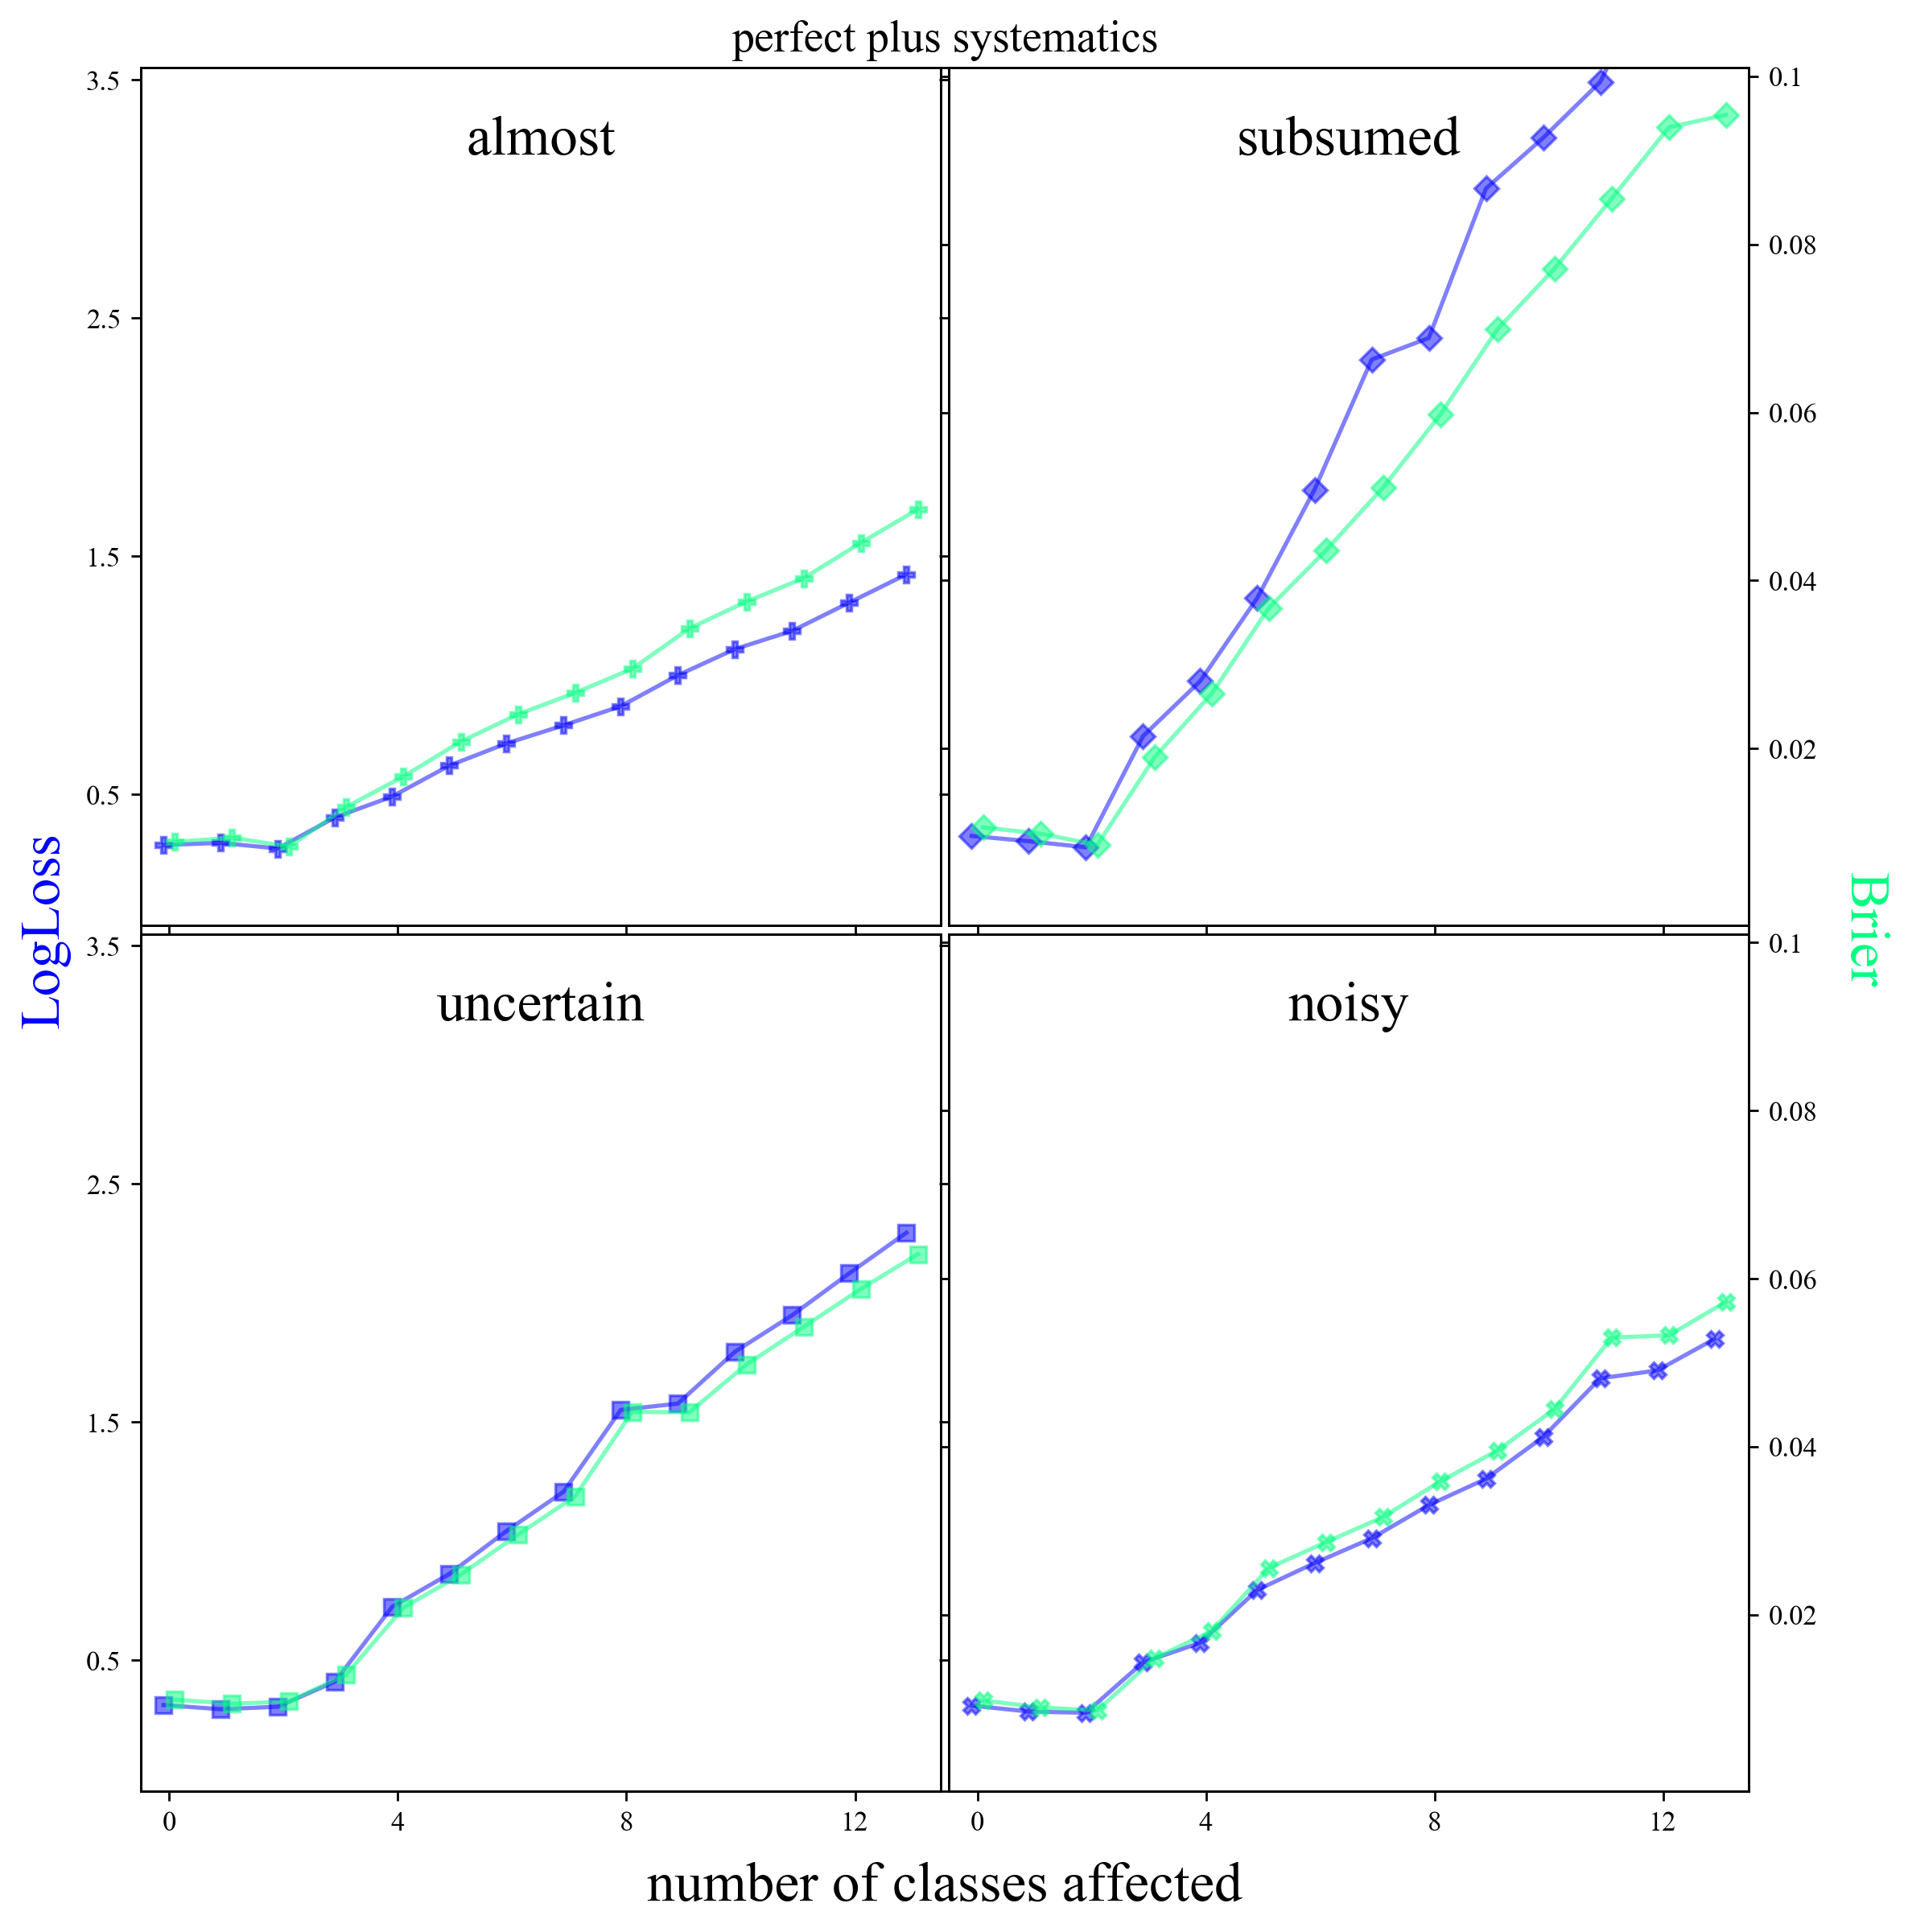
\includegraphics[width=0.5\textwidth]{./fig/systematics_onlyperfect.png}
%		\caption{\aim{After much iteration on how best to present these tests, a figure similar to Figure~\ref{fig:cruise} but for the tunnel vision classifier (heading) on different baseline classifications (panels) as a function of weight on the affected class (rather than number of classes) is under construction.}}
%		\label{fig:tunnel}
%	\end{center}
%\end{figure}





\subsection{Representative classifications}
\label{sec:realresults}

\begin{figure*}
	\begin{center}
		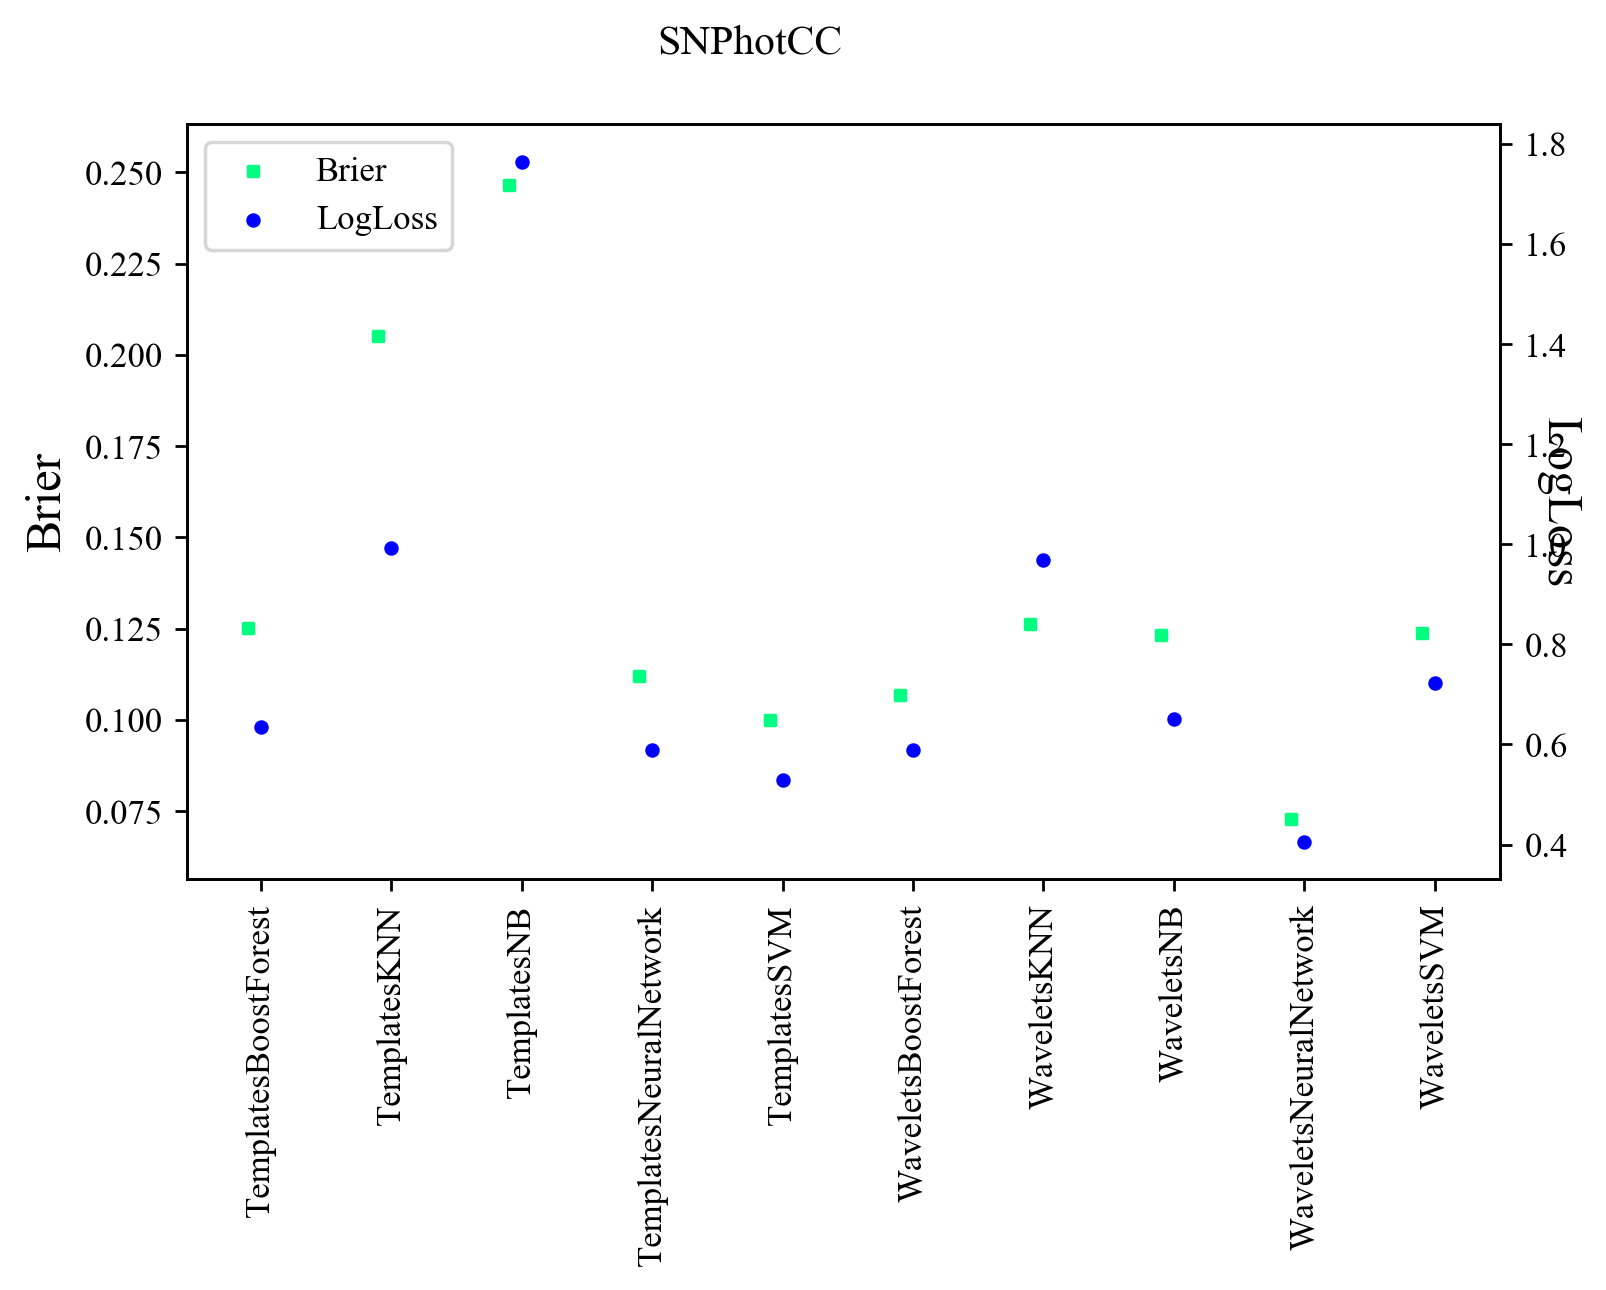
\includegraphics[width=0.85\textwidth]{./fig/SNPhotCC_res.png}\\
		 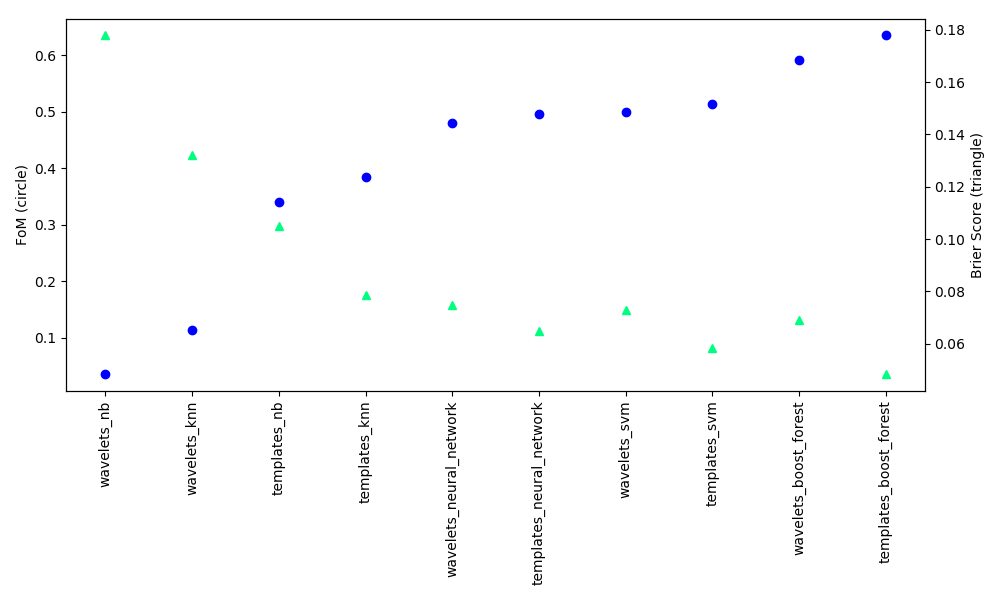
\includegraphics[width=0.8\textwidth]{./fig/fom_vs_brier.png}
		\caption{The algorithms presented in \cite{lochner_photometric_2016} based on a representative subset of the SNPhotCC data.
		The top panel shows the performace of the various classification schemes described in \ref{sec:realdata} as a function of both the Brier and log-loss scores.
		The bottom panel shows the performance of the same classification schemes, this time evaluated on the SNPhotCC Figure of Merit (explicitly defined in Section~\ref{sec:past}) which is based on a combination of pseudopurity and classification efficiency.
		The Figure of Merit closely tracks the Brier score for the same entries, suggesting its applicability to the problem of photometric transient classification.
		\label{fig:real_metric_compare}}
	\end{center}
\end{figure*}

%\textbf{Current plan is that we compute the SNPhotCC metric for Michelle's contributions and also turn the binary classifications into probabilities - Renee will flesh this out}
%\aim{We are still iterating on the most informative tests to conduct on the \snphotcc\ data.
%I would like to have the confusion matrices from a real classification challenge (\snphotcc\ or Ashish Mahabal's) and test different weightings of our metrics on mock classification probabilities derived from those confusion matrices to check whether we choose the same ``winner,'' but the arrangements have not yet been finalized.
%The ``pipeline,'' however, is complete and ready to run as soon as the test conditions are agreed upon.}


% \subsection{Weighting systematics}
% \label{sec:weight_res}
%
% \aim{We have not yet reached consensus on what tests are reasonable in the absence of physical motivations, as the test cases here are independent of such context.}
